\documentclass[12pt]{report}
\usepackage[a4paper, left=1in, right=1in, top=1in, bottom=1in]{geometry}
\usepackage{xcolor}
\usepackage{amsmath}
\usepackage{amsthm}
\usepackage{amssymb}
\usepackage{amsfonts}
\usepackage{algpseudocode}
\usepackage{mathtools}
\usepackage{xcolor}
\usepackage{float}
\usepackage{framed}
\usepackage{listings}
\usepackage{graphicx}
\usepackage{subcaption}
\usepackage{tikz}
\usetikzlibrary{arrows, positioning}

\lstset{basicstyle=\ttfamily,
  commentstyle=\color{red},
  keywordstyle=\color{blue},
  %basicstyle=\footnotesize,
  frame=lines,
  numbers=left,
  stepnumber=1,
  showstringspaces=false,
  tabsize=1,
  breaklines=true,
  breakatwhitespace=false,
}
\usepackage{hyperref}
\hypersetup
{
    colorlinks=true,
    linkcolor=blue,
    filecolor=magenta,
    urlcolor=cyan,
    pdftitle={\Huge \textbf{CS218 Solutions}},
    pdfpagemode=FullScreen,
}
\usepackage[utf8]{inputenc}
\usepackage{graphicx}
\usepackage{longtable}
\usepackage{multirow}
\usepackage{enumitem}
\setlength{\parindent}{0pt}

\begin{document}
\subsection*{\huge\bfseries Binary Search and Variants}
\begin{enumerate}[label=\textbf{\arabic*.}]

  \item We first need to find a range before performing binary search. For this we can drop the egg at 
  floors 1,2,4,8,\dots until it breaks. If $2^n \leq h < 2^{n+1}$, the egg breaks at the $(n+1)^{th}$
  drop and $n+1 = \lfloor \log_2 h \rfloor + 1$ which is $O(\log h)$. Now we can binary search in the range from
  $2^n$ to $2^{n+1}-1$. The range is $O(2^n)$ so the binary search will take $O(\log 2^n) = O(n) = O(\log h)$
  egg droppings, so overall it's still $O(\log h)$.

  \item Whenever we want to find subarray sums, it is useful to precompute a prefix sum array, which is
  has the sums of the first $i$ elements i.e. $[0, a_1, a_1+a_2, \dots, a_1+a_2+\dots+a_n]$. This takes 
  $O(n)$ time to calculate as the $i^{th}$ prefix sum is obtained by adding an array element to the $(i-1)^{th}$
  prefix sum. With these prefix sums, any subarray sum from $a_i$ to $a_j$ is obtained by subtracting the prefix
  sum to $a_{i-1}$ from the prefix sum to $a_j$. Now for every $i$, we can binary search the subarray sums
  starting from $a_i$, to get the least $j$ such that sum from $a_i$ to $a_j$ is at least $S$. This is 
  possible as sum from $a_i$ to $a_j$ is an increasing function w.r.t $j$. So for every $i$, we will take
  $O(\log n)$ time and hence the final time complexity is $O(n \log n)$.

  Another method is to binary search for the minimum length directly. For fixed subarray length, finding the
  maximum subarray sum takes $O(n)$ time. Just find the sum for the first subarray, and for the next subarray,
  add the new element and subtract the first element. So this is just a 1 time traversal of the array. Now we 
  need $O(\log n)$ queries to narrow down the fixed length by binary searching for first length where the subarray
  sum is at least $S$. Each query takes $O(n)$ time so our time complexity is $O(n \log n)$.

  Turns out this question can be solved in $O(n)$ time itself. The idea is to have 2 pointers, one for the start 
  of the subarray and one for the end of the subarray. For every start index, keep moving the end value until 
  the sum of the subarray is at least $S$. Once that's reached, move the start pointer 1 step forward and repeat. Note that 
  this would give the smallest subarray for every start index, as the end index will never need to decrease whenever 
  the start index moves forward. Updating subarray sum is also easy whenever a pointer moves, just correct for
  the new element added/deleted. This algorithm is $O(n)$ as each pointer moves at most $n$ times, they are initialized as 
  the beginning of the array.

  \item We just need to find the $n^{th}$ and $(n+1)^{th}$ element of the merged array. For now, let's just assume 
  that the $n^{th}$ element is in the first array and try to find it. How to check if the $i^{th}$ element of the 
  first array is the $n^{th}$ element of the merged array? We know it's greater than exactly $i-1$ elements in the
  first array, so it has to be greater than $(n-1)-(i-1)$ elements in the second array, as it overall has to be greater
  than $n-1$ elements. So we just check that, it should be greater than the $(n-i)^{th}$ index and smaller than $(n-i+1)^{th}$
  index of the second array, if so we have found it. If it's too small i.e lesser than the $(n-i)^{th}$ element of 
  the second array. We need to check from $(i+1)$ to $n$ in the first array. If it's too big, we need to search from $1$ to 
  $i-1$ in the first array. So we can binary search, dividing the search space by half in each time. Suppose we don't
  find the $n^{th}$ element in the first array, we check the second array for it. Similarly we can find the $(n+1)^{th}$
  element by checking both arrays.

  \item We first sort the array taking $O(n \log n)$ time. Now for each element $x$ in the array, binary search for $S-x$.
  This also takes $O(n \log n)$ as we binary search $n$ times.
  
  After sorting, there is also an $O(n)$ approach. Keep 2 pointers at start and end. If the first and $n^{th}$ element
  sum greater than $S$, we know that the $n^{th}$ element can never be part of a pair, it's too big even when paired 
  with the first element. So we discard it from our search by decrementing our end pointer. If the sum was smaller than 
  $S$, similar logic follows and we increment our start pointer. We keep doing this until we either get a sum $S$ or 
  our pointers clash. Since the distance between them is always decreasing by 1 step this is $O(n)$

  \item Since the derivative is an increasing function, we can find where it has a root by doing something like bisection
  method. We first find an interval where the root is, suppose we check a random point $a$ and $f'(a)$ is negative.
  We then check $f'(a+1), f'(a+2), f'(a+4), \dots$ until we get a point where the derivative is positive, to
  locate our interval. Once we have a start and endpoint, we check the derivative at the midpoint and based on 
  its sign, we half the interval search each iteration, increasing the number of bits of precision each time by 1.

  \item The smallest base is $2$ so the highest exponent is $\log_2 a$. For each exponent $k$, we binary search for $b$
  to get $b^k$ to be $n$. So we need $O(\log a)$ queries to get $b$ for each $k$, if it exists. But how much time
  does each query take. Assume the naive human multiplication method, multiplication take $O(d^2)$ time where $d$
  is the number of digits. Since we only multiply till a size of $a$, we have $O(\log a)$ digits. We multiply
  almost $O(\log a)$ times to do exponentiation so each query is $O(\log^3 a)$. This makes binary searching for a 
  fixed exponent as $O(\log^4 a)$. So our final time complexity if $O(\log^5 a)$. This algorithm can be make a lot 
  faster by using more efficient methods for multiplication and exponentiation, but eh.

  \item The highest value of $f$ is just $\left \lfloor \frac{a_1 + \dots + a_n}{n} \right \rfloor$. This is clearly
  achievable by making everyone having anything above this value give off their land one by one. This process will 
  terminate as everyone can't have land below the average. Anything above this isn't achievable as if everyone has 
  above the average, the total area of land will not be sufficient.

  For the second part, we first sort the array, and calculate prefix and suffix sums (sums of the first $i$ elements
  on either sides). This overall takes $O(n \log n)$ time. Now for a fixed value of $f$, we first binary search for 
  $f$ in our array to find how many elements are less than $f$. The extra land we need is summation of [$f - $ 
  element lower than $f$]. This is just $f \times$ (no of elements lower than $f$) $-$ the corresponding prefix sum.
  Now for any value of $c$, we can also get the extra land we get, it's equal to corresponding suffix sum - $c \times$ 
  (no of elements higher than $c$). Let us first find between 
  which 2 numbers in the array does $c$ lie. $c$ doesn't have to be a number in the array, but we can binary search 
  assuming that for now. Choose an element in the array as $c$, and calculate the land we get, if it's too much, 
  choose a larger element as $c$, and if it's too large, choose a smaller element as $c$. At the end of the binary 
  search, we can tell between which 2 numbers in the array $c$ is. Once we have this, we can actually solve for $c$, 
  as we have the equation: 
  \[ \text{suffix sum} - c \times \text{no of elements higher than $c$} = f \]
  We know all the quantities except $c$, so we can get $c$. 

  \item Walk to $2^k$ and back to $0$, $-2^k$ and back to $0$. Do this for every $k$ from $0$ until you find the
  treasure. If the treasure is at $N$ and $2^{n-1} < N \leq 2^n$, we walk a distance of $4(1+2+4+\dots+2^n) = 
  4(2^{n+1} -1) < 16(2^{n-1}) < 16N$, so we walk $O(N)$ distance.

  \item $\log(n!) = \sum_{i=1}^{n} \log(i) \geq \log(n/2+1) + \log(n/2+2) + \dots + \log(n) \geq \log(n/2) + \log(n/2) 
  + \dots + \log(n/2) = (n/2) \log(n/2) = (n/2) (\log n - 1) = (1/2) n \log n - n/2$

  \item The inequality can be formed by comparing a riemann sum (area of rectangles) with the integral of $\log(x)$
  \begin{figure}[H]
    \centering
    \includegraphics[width=0.5\textwidth]{logxGraph.png}  
  \end{figure}
  So $\log(n!) = \sum_{i=1}^{n} \log i \geq \int_{1}^{n} \log x \ dx = [x \log x - x]_1^n = n \log n - n + 1$

  \item 
  \begin{itemize}
    \item True as $2n+3 \leq n^2$ for large $n$
    \item False, $\sum_{i=1}^{n} i^2 = \frac{n(n+1)(2n+1)}{6} = \Theta(n^3) > O(n^2)$
    \item True, will be proved in Q15 
    \item False, $n^n = 2^{n \log n} > O(2^n)$
    \item False, $2^{3n} = {(2^n)}^3 > O(2^n)$
    \item True, ${(n+1)}^3 \leq {(n+n)}^3 = 8n^3 = O(n^3)$
    \item True, ${(n+\sqrt{n})}^2 \leq {(n+n)}^2 = 4n^2 = O(n^2)$
    \item True, $\log(n^3) = 3 \log n = O(\log n)$
  \end{itemize}

  \item Out of syllabus
  \item Out of syllabus
  \item Out of syllabus
  \subsection*{\huge\bfseries Reducing to a Subproblem}
  \item The same rectangle trick can work for both bounds
    
  \begin{figure}[htbp]
    \begin{subfigure}{0.5\textwidth}
      \includegraphics[width=\linewidth]{1stinequality.png}
    \end{subfigure}%
    \begin{subfigure}{0.5\textwidth}
      \includegraphics[width=\linewidth]{2ndinequality.png}
    \end{subfigure}
  \end{figure}

  Solving integrals, we get $\log(n+1) \leq \sum_{i=1}^{n} 1/i \leq 1+\log(n)$

  \item If we are selling it on day $i$, in order to maximize profit, we have to have bought it at the cheapest
  price that came so far. So what we can do is maintain the cheapest price (minimum) we have seen so far. Now we 
  just assume we sell on day $i$ to get the best profit for that day, and compare it with the best profit we have 
  seen so far. So an extra subproblem we are solving is the minimum price we have seen so far.

  \item With each question, we can eliminate 1 person from our search group. Let's say we ask $i$ if she knows $j$.
  If $i$ doesn't know $j$, $j$ is not the celebrity as the celebrity is known by everyone. If $i$ knows $j$, $i$ isn't
  the celebrity as the celebrity doesn't know anyone. So we need just $n-1$ queries as we eleminate 1 person each time.

  \item We can do this by thinking backwards. Our last step is probably adding $a_0$ to $a_1 \alpha + \dots + a_{n-1} 
  \alpha^{n-1}$. And to get the second term, our last step is probably multiplying $\alpha$ to $a_1 + a_2 \alpha + \dots 
  + a_{n-1} \alpha^{n-2}$ as $\alpha$ factors out. But this is great, as now this term is the same question but with 
  $n-1$ terms, we have got the relation $T(n) = T(n-1) + 2$. Here's how the computation looks for 3 terms: $a_0 + 
  (\alpha \times (a_1 + (\alpha \times (a_2 + (\alpha \times a_3)))))$
  
  \item Let's convert this to some sort of a graph problem. For each $i$ in the domain, let's draw a directed edge
  to $f(i)$. Since each number has 1 and only 1 outgoing edge, our graph only has cycles, and chains which merge into
  a cycle.

  \begin{figure}[ht]
  \centering
  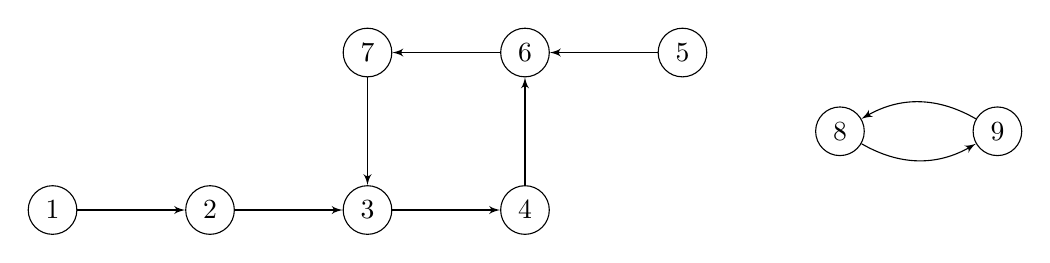
\begin{tikzpicture}
    \tikzset{vertex/.style = {shape=circle,draw,minimum size=1.5em}}
    \tikzset{edge/.style = {->,> = latex'}}
    % vertices
    \node[vertex] (1) at (0,0) {1};
    \node[vertex] (2) at (2,0) {2};
    \node[vertex] (3) at (4,0) {3};
    \node[vertex] (4) at (6,0) {4};
    \node[vertex] (5) at (8,2) {5};
    \node[vertex] (6) at (6,2) {6};
    \node[vertex] (7) at (4,2) {7};
    \node[vertex] (8) at (10,1) {8};
    \node[vertex] (9) at (12,1) {9};
    %edges
    \draw[edge] (1) to (2);
    \draw[edge] (2) to (3);
    \draw[edge] (3) to (4);
    \draw[edge] (4) to (6);
    \draw[edge] (6) to (7);
    \draw[edge] (7) to (3);
    \draw[edge] (5) to (6);
    \draw[edge] (8) to [bend right] (9);
    \draw[edge] (9) to [bend right] (8);
    \end{tikzpicture}
    \caption*{Example Graph Picture for $n = 9$}
  \end{figure}

  Take the example above as our question. Clearly numbers like $1, 5$ can't be in our set, as nothing maps to them. Can
  $2$ be in our set? Also no, as since $1$ isn't in our set, nothing maps to $2$. We can apply this reasoning many times, 
  all linear chains, which aren't part of any cycle can't be in our set. And the remaining elements obviously satisfy our 
  condition, as in every cycle there is 1 ingoing and outgoing edge for every number.

  The algorithm to get the set can be like this: first create an frequency array holding how many times each number is an 
  image. Then add all the numbers which have no image (value 0 in the array) into a queue. Now we dequeue $i$, and basically
  mark it as not in solution set. We also have to decrease the frequency of $f(i)$, as $i$ is deleted. If $f(i)$'s frequency 
  decreases to 0, we add $f(i)$ to our queue, it also has to be deleted (this corresponds to the case where $f(i)$ is also in 
  a chain). We keep doing this until our queue is empty, and the elements we never visited are the ones in our final answer.

  \item We can first sort all the intervals in ascending order of left endpoint. If left endpoints are equal, sort in 
  descending order of right endpoint. This ordering has the following objective. No interval can be contained by an interval
  after it, so it becomes easier to deal with (assuming all intervals are distinct). Now we can go one by one in this 
  interval list. If we are at interval $i$, we don't have to care about later intervals, it won't be contained in them.
  In the intervals before $i$, they will contain $i$ on the left side for sure, if any of them have the right endpoint 
  greater than  or equal to $i$'s, $i$ is contained, else it is not. So all we have to do is maintain the greatest right 
  endpoint found so far. If it's $\geq i$'s endpoint, $i$ is contained, else it isn't. And then update the greatest endpoint 
  found so far. So overall the algorithm is $O(n \log n)$ (sorting) + $O(n)$ (single traversal of the array).

  \item Let's say we wanted to calculate for $n = 4, k = 2$ which is $ab + ac + ad + bc + bd + cd$. We can actually group 
  this based on whether $d$ is a term or not, so it becomes $d(a + b + c) + (ab + ac + bc)$. But these are subproblems, $n = 3, k = 1$
  and $n = 3, k = 2$. We can generalize this recursive idea, $f(n, k) = a_n(f(n-1, k-1)) + f(n-1, k)$ by choosing whether 
  $a_n$ is part of the terms or not. Our base cases are $f(1,1) = a_1$, $f(n,1) = a_n + f(n-1,1)$. We can just create an 
  $n \times k$ grid and calculate $f(i,j)$ and fill it in each cell, going in increasing order of $i$ and increasing order 
  of $j$ (there are more efficient ways space complexity wise but eh).

  We can also achieve this recursion logically, not only just by mere observation. As per the hint, the given entity is the coefficient of $x^{n-k}$ in the polynomial $\prod_{i=1}^{n} (x + a_{i})$. Rewriting as $[\prod_{i=1}^{n-1} (x + a_{i})]*(x + a_{n}) = x*[\prod_{i=1}^{n-1} (x + a_{i})] + a_{n}*[\prod_{i=1}^{n-1} (x + a_{i})]$, we see that coefficient of $x^{n-k}$ in $\prod_{i=1}^{n} (x + a_{i})$ in LHS = sum of coefficients of $x^{n-k-1}$ in $\prod_{i=1}^{n-1} (x + a_{i})$ and $x^{n-k}$ in $a_{n}*\prod_{i=1}^{n-1} (x + a_{i})$ in RHS. Hence we get the recursion equation above.

  \subsection*{\huge\bfseries Divide and Conquer}

  \item This question is very similar to the interval containment problem. We consider $(a, b)$ to contain $(c, d)$ if $a \leq c$
  and $b \geq d$, but dominate $(c, d)$ if $a \geq c$ and $b \geq d$. So the solution is again like this: sort in decreasing order 
  of first coordinate, if it's equal decreasing order of 2nd coordinate. Then it's a single traversal of the array, by maintaining 
  the max of the 2nd coordinate seen so far. If it's $\geq$ the current 2nd coordinate, the current point is dominated, else update the 
  max of 2nd coordinate.

  \item It's been given that the majority fingerprint occurs more than $n/2$ times. So if we split the array into 2, we
  can say in at least one of the array, the fingerprint occurs more than $n/4$ times, and hence is the majority fingerprint for 
  that subarray too. This observation is useful for a divide and conquer idea.

  Let's say we have solved the subproblems for the two $n/2$ size arrays, and have kept the majority fingerprint of each subarray
  at the beginning of them respectively. One of these fingerprints is going to be our final solution itself. We can just check how 
  many times each one appears. Traverse both subarrays, and manually count how many times you see each of our candidate solutions.
  Whichever you see more is our final solution, and keep it at the beginning of the whole array. This method will satisfy 
  $T(n) = 2T(n/2) + O(n)$ so $T(n)$ is $O(n \log n)$.

  \item We use a balanced BST for this. But we also store one extra thing in each node, the number of elements in the subtree with
  root as that node. How do our functions for insert, delete, rotate change in order to maintain this data? While inserting, we just 
  add 1 to every node on the path from the root to the new node. For deleting, we just subtract 1 from every node on the path to the
  node to delete. Balancing is also not that hard; as we exchange subtrees between nodes, we also have to just exchange the data
  which maintains the number of elements. But what's the point of maintaining this data? It helps us to find the number of elements 
  smaller than a query in $O(\log n)$ time. Take the same path as if you are inserting the query. If you take a right turn, you know the 
  root and the left subtree are all smaller than the query. If you take a left turn, the root and the right subtree are all larger than 
  the query, so you have to add $1 + $ size of right subtree to your answer. Just keep doing this until you get to a leaf.

  How do we use this data structure? We can iterate through the array and maintain this special BST of all elements we have seen, 
  seen so far. Say we are at $A[j]$ we have to find number of $i < j$ and $A[i] > 2A[j]$. This is basically number of elements in the 
  BST which are greater than the query $2A[j]$ which can be found in $O(\log n)$ time. And then we have to insert $A[j]$ which also takes
  $O(\log n)$ time.
  So this algorithm will take $O(n \log n)$ time.

  \item Think about shading the visible parts of each line. If you move from left to right, the lines will be in increasing order of slopes,
  and form a sort of U shape. So we can start off by first sorting in increasing order of slope. If 2 lines have same slope, the one with 
  smaller `c' is redundant. Now we're going to traverse this array one by one, and maintain a list of lines which are visible. Note that in 
  this list, except for the first and last line, only line segments are visible. Now a crucial observation is that the next line will intersect
  only 1 of the visible parts, as it's slope is greater than the whole thing. And which part it insersects can be found by binary search. 
  
  Let's check if line $l$ intersects $vis[i]$ (in the visible part of it). For this, it should intersect between the endpoints of the visible
  part, $vis[i-1]$ and $vis[i]$'s intersection, $vis[i]$ and $vis[i+1]$'s intersection. Let's call these endpoints, $a$ and $b$, and $l$'s
  insersection point with $vis[i]$ as $x$. If the order of points of line $vis[i]$ is $p, a, b$, then line $l$ intersects with something 
  before $vis[i]$. If the order, is $a, b, p$, then the line insersects with something after $vis[i]$. So in this way we can binary search, 
  by dividing our search space. Once we found out which line it intersects with, all the lines in the array after it are to be neglected, they
  will be hidden. We don't have to spend time deleting them, just store an endpointer to $vis$ to save time. Overall the time complexity is 
  $O(n \log n) + n \times O(\log n) = O(n \log n)$.

  \item This question is very similar to the previous one, just turning it upside down. So we can do the same process, sort the lines in decreasing
  order of slopes, and iterate through this array. However here, we also have the additional constraint that $y \geq 0$, so the starting and ending
  lines also terminate. But stil, we follow the same process, and in the end, finding the vertices from the lines is easy. This is overall
  $O(n \log n) + O(n) = O(n \log n)$.

  \item Out of syllabus
  
  \item Let's divide our array into 2 subarrays, left half and the right half. Let's say we have already solved the subproblems within the 2
  halves, now all that's left is to count number of significant inversions where $i$ is in the first half and $j$ is in the second half. In order to 
  do this is $O(n)$ let's assume some preprocessing is already done for us, the left subarray and the right subarray are already sorted. This will
  make our counting easier, and it's now like we are doing our counting while doing a mergesort.
  
  Keep pointer $p_1$ at the start of the first array, and $p_2$ at the start of the second array. We just want to find for every $i$, how many $j$
  are there such that $A[i] > 2A[j]$. So for $p_1$ pointing to $i=0$, keep moving $p_2$ until the condition isn't satisfied. The number of $j$'s for 
  $i=0$ are the number of times $p_2$ moved. Now increment $p_1$, and continue moving $p_2$ whenever $A[i] > 2A[j]$, for the new $i$, the total number 
  of significant inversions is total number of times $p_2$ moved. We can keep doing this for all values, until both pointers reach the end. This takes 
  $O(n)$ time. But our subroutine isn't done, we have to now merge these 2 subarrays to give a sorted full array, but this also takes only $O(n)$ time.
  So we have the recursion $T(n) = 2T(n/2) + O(n)$ so $T(n) = O(n \log n)$.

  \end{enumerate}
\end{document}